% Chapter 1

\chapter{Introduction} % Main chapter title

\label{Chapter1} % For referencing the chapter elsewhere, use \ref{Chapter1} 

%----------------------------------------------------------------------------------------

% Define some commands to keep the formatting separated from the content 
\newcommand{\keyword}[1]{\textbf{#1}}
\newcommand{\tabhead}[1]{\textbf{#1}}
\newcommand{\code}[1]{\texttt{#1}}
\newcommand{\file}[1]{\texttt{\bfseries#1}}
\newcommand{\option}[1]{\texttt{\itshape#1}}

%----------------------------------------------------------------------------------------

\section{Parental controls}

\subsection{Overview}
Parental controls developed in the digital era as a means to allow parents to restrict the access of content to their children and may be included in digital television services, computer and video games and mobile devices. The content may not be appropriate for their age and is aimed more at adult audiences. The characteristics of inappropriate content depends for each parent, and is also correlated with the child's age and maturity level and includes information and images that can upset the child, inaccurate information or information that can cause dangerous behavior. Some of this content could be:

\begin{itemize}
\item pornographic material
\item content containing swearing
\item sites that encourage vandalism
\item pictures, videos or games which shows images of violence
\item gambling sites
\item unmoderated chatrooms
\end{itemize}

It is very easy for the child to stumble upon unsuitable sites by accident on any internet enabled device, like mobile phone or tablet and it can be difficult to monitor and filter the content. \parencite{innapropriateContent}

Parental control solutions fall into four categories:

\begin{itemize}
\item content filters, which limit access to different types of inappropriate content
\item usage control, which works by constraining the usage of certain devices by placing time-limits on usage or forbid some types of usage
\item computer usage management tools, which enforces the use of certain software
\item monitoring, which can track the activity when using the devices
\end{itemize}

The rising availability of the Internet increased the demand for methods of parental control that restrict content. Mobile phones offer the most convenient and constant method for content access, and teens ages 13 to 17 are going online frequently. A study by Pew Research Center found that 92\% of teens report going online daily, 24\% of which are using the internet almost constantly, 56\% going online several times a day and 12\% reporting once a day use. Only 6\% go online weekly and 2\% less often. \parencite{lenhart2015teens}

\begin{figure}[th]
\centering
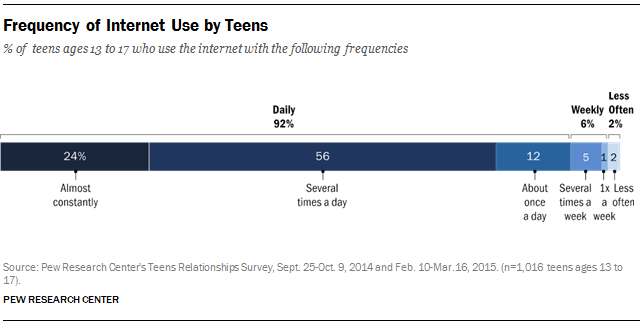
\includegraphics[width=1\textwidth]{Figures/frequency-of-internet-use-by-teens}
\decoRule
\caption[Frequency of Internet Use by Teens]{Frequency of Internet Use by Teens}
\label{fig:frequency-of-internet-use-by-teens}
\end{figure}

The same study finds that nearly three-quarters have or have access to a smartphone and only 30\% have a basic phone and 12\% of teens 13 to 17 have no cell phone of any type.

\subsection{Techniques}

There are two types of control techniques, behavioral control, which consists of controlling the amount of time and how much the child can view, and psychological control, which involves parents tying to influence children by affecting their emotional side by manipulating or insensitivity. Adult control can be divided into three prototypes, each of which has influenced greatly the child-rearing practices \parencite{baumrind1966effects}:

\begin{itemize}
\item permissive: the parent attempts to behave in a nonpunitive, acceptant and affirmative manner and consult with the child about policy decisions and gives explanations for rules
\item authoritarian: the parent attempts to shape, control and evaluate the behavior of the child in accordance with a set standard of conduct, by valuing obedience as a virtue and favoring punitive, forceful measures to curb self-will
\item authoritative: the parent attempts to direct the child's activities in a rational manner, by sharing the reasoning behind the policy and soliciting the child's objections when he refuses to conform; disciplined conformity and autonomous self-will are valued by the authoritative parent
\end{itemize}

Several techniques exists for creating parental controls to block certain websites. Parental control software can monitor API to observe applications such as web browsers or chat applications and to intervene based on certain criteria, such as time based criteria or as a match in a database of banned words. Other techniques that involve a proxy server are also used, in which the proxy server serve as an intermediary which can intervene in the delivery of some content based on various criteria based on the content, but this method has a major disadvantage because it requires client configuration to use the service, which can be easily bypassed.

The difference between content filters and computer usage management methods is that the later is focused on empowering the parents to balance the computing environment for children, by allowing parents to enforce the learning component into the computing time of children, where children can earn play time by working through educational content. This method is very powerful because it stimulates self-regulation in children, instead on relying solely on parental control, and we will use some ideas from this method to develop our control and regulation system.

Recently, some devices which are used for network based parental control have emerged. These devices use different methods to block inappropriate content, such as packet filtering, DNS Response Policy Zone (RPZ) and Deep packet inspection (DPI), and work as a firewall router. Some commercial and governmental communication networks use these methods also, but these type of devices were developed for home also, and are used to create a new home wireless network specifically designed for kids to connect to. We developed our system using the same approach, by creating a custom wireless network for different type of users, different age level children and parents, and by using the packet filtering and DNS techniques to manage content filters.

\subsection{Content filters}

The increased use of mobile devices has created a demand for parental controls for these devices. The first carrier which offered age-appropriate content filters was Verizon, in 2007. With the release of iPhone OS 3.0 in 2009, Apple introduced a mechanism to create age brackets for users, to block unwanted applications from being downloaded. Filtering options are also offered by most internet providers, to limit internet browsing options and block unsuitable content. The software used to restrict or control the content a user is capable to access is commonly referred to as internet filter or content filter.

The content access restrictions can be applied at different levels, from governments applying them nationwide, to ISP blocking it's clients and by a parent to a child's computer. The implementation of this content filtering mechanism can be done at different levels also, by software on the client computer, by using the network infrastructure such as proxy servers, DNS servers or firewall, but none of these solutions alone provides complete coverage, so a mix of technologies have to be used to achieve proper content control.

\begin{itemize}
\item Browser based filters are the most lightweight solution, and the filtering is done by using a third-party browser extension
\item E-mail filters are commonly implemented using a statistical method, Bayesian filters, by acting on information contained in the mail body, headers or attachments
\item Client side filters work by installing it as software on each target device
\item Content-limited (or filtered) ISPs
\item Network-based filtering
\item DNS-based filtering
\item Search-engine filters
\end{itemize}

%----------------------------------------------------------------------------------------

\section{A self regulation approach}

%----------------------------------------------------------------------------------------
